\section[Unclusterfuck]{How to unclusterfuck code}

% what allows us to design CPUs is that we have a good theory of what the world is like. This allows us to construct things in our mind before testing whether those abstractions worked.
% This is the basis of all modern technology.

\frame{
	\begin{center}
		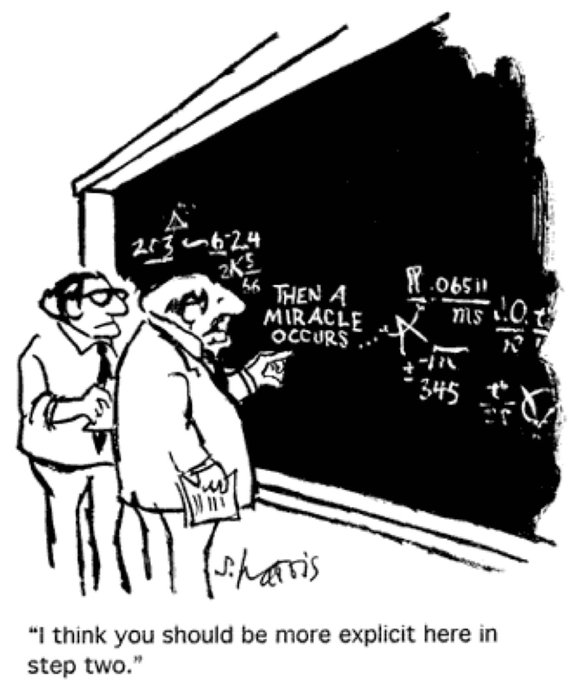
\includegraphics[height=0.76\textheight]{miracle.jpg}
	\end{center}
	\cite{thenamiracleoccurs}
}

\note{
	\begin{itemize}
		\item It will happen to you. You will have to unclusterfuck code. Probably your own, because later in the code, you'll have hindsights you didn't have before.
		\item How to do that in a practical manner?
	\end{itemize}
}

\frame{
	\begin{center}
		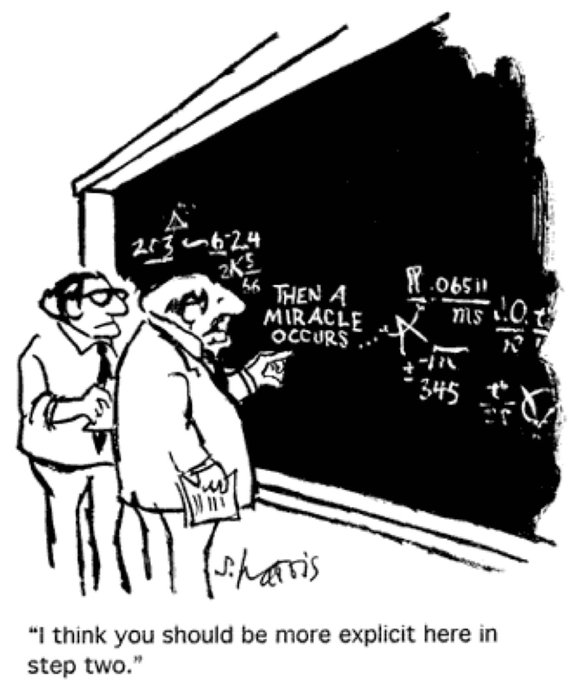
\includegraphics[height=0.76\textheight]{miracle.jpg}
	\end{center}
	\cite{thenamiracleoccurs}
}

\note{
	\begin{itemize}
		\item First, you fix any typos in comments, if available
		\item Then in variables, if named after some scheme.
		\item Then try to find variables code like \texttt{varname[5]} and give it a name that you think it may represent.
		\item First the one that is occuring the most first.
		\item Then the next common one and so on.
		\item Then try playing around, checking if the your interpretation of the code makes sense, and fix variable names until their use in the code  maps fully to your mental model of the code
		\item Then, if its a long function, split it into parts. Look at code that looks similiar, and try to outsource it into a generalized function that does what you want the snippets to do. Give it a clear name of what it does, and replace the duplicate code.
		\item Also, use guard clauses:
\begin{verbatim}
	if(a) {
		if(a) {
			if(a) {
				your_code();
			}
		}
	}

	->

	if(!a) {
		log("a is not the case");
		return;
	}

	if(!b) {
		log("b is not the case");
		return;
	}

	if(!c) {
		log("c is not the case");
		return;
	}

	your_code();
\end{verbatim}
		\item Do this repedeatly, so that no code that does basically the same thing exists twice anywhere. And check whether the function name really describes what it does.
		\item Add assertions, exceptions and debug stuff as well.
		\item Each error that occurs to you while testing must have a reasonable response that you intelligently chose. 
		\item There are states where your software may be unable to recover, and needs to crash (better crash than faulty data that looks like it's reliable). But it should crash gracefully and produce a log file.
		\item And this case should only be the last resort out of technical neccessity, and only for things you have no control over, like \texttt{fork} returning -1, or the hard disk being full. Never for anything you have control over, because you stopped stuff from going from in your software and report every warning or error, each of which you fix, with the strictest compiler settings available.
		\item After that, the code will be \textit{very} readable, and work, and even notify when other parts use it wrongly, by the newly added assertions and warnings.
	\end{itemize}
}
